\subsection{Model Optimizations} \label{subsec:mdopti}
 In this section we will review different approaches to reduce the size and the computational complexity of a model which can be an issue when implementing on \acrshort{fpga}. Moreover, \textcite{nurvitadhi_can_2017} believe that sparsity exploitation (see section \ref{subs:pruning}) and extremely compact data types (see section \ref{subs:quantization}) will become the norm in the next-generation \acrshort{cnn}.
\subsubsection{Efficient Model Design}
The size of the model can be reduced by changing the architectures of the models. As many approaches have been proposed, we focus our interest on architectures that target the embedded space.

SqueezeNet \cite{iandola_squeezenet_2016} uses an architecture similar to AlexNet and replaces all layers (except the first and last one) by \textbf{Fire Module}. The \textbf{Fire Module} is a building blocks where the convolution filter is composed of two layers. The first one (squeeze block) is composed only of $1 \times 1$ filters, which squeezes the number of channel to reduce the number of computation in the next block. The second (expand block) one is composed of $1 \times 1$ and $3 \times 3$ convolutions. We can reduce with this method the number of parameters of AlexNet from $240$MB to $4.8$MB. The number of parameters can even be reduced to $0.47$MB with no loss of accuracy from the baseline AlexNet method by applying Deep Compression \cite{han_deep_2016}. However, it has a big memory footprint, is slower in runtime and consumes more energy than AlexNet \cite{sze_efficient_2017}.

NasNet \cite{zoph_learning_2018} uses a search method, \acrfull{nas}, to find good convolutional architectures on a dataset of interest. A controller recurrent neural network saloes child networks with different architecture. The learned architecture is flexible as it may be scaled in terms of computational cost. However the resulting network ends up very complex \cite{sandler_mobilenetv2_2019}.

MobileNet \cite{howard_mobilenets_2017} uses \acrshort{dsc}, described in section \ref{subs:dsc}, to build small and low latency models that can be matched to the design requirements. It sets also 2 hyper-parameters to set the model size and throughput: width multiplier $\alpha \in [1; 0[$, which reduces the number of input and output channel at each layer, and resolution multiplier $\rho \in [1; 0[$,  which reduces spatially the input and output \acrshort{fm} at each layer.

ShuffleNet \cite{zhang_shufflenet_2018} is a computation-efficient architecture designed for mobile devices with very limited computing power. It reduces computation cost while maintaining accuracy by using \textbf{pointwise group convolution} which reduces computation complexity of $1 \times 1$ convolution. It uses also \textbf{channel shuffle} on the channels such that \textbf{group convolutions} obtain information from different groups. Then more powerful structures can be build with multiple group convolutional layer. However, the group convolutions and the bottleneck structures add \acrshort{mac} which is a non-negligible cost \cite{ma_shufflenet_2018}. The group convolution contributes to network fragmentation and reduce parallelism. Moreover, the "Add" operation is non-negligible too.

MobileNetV2 \cite{sandler_mobilenetv2_2019} is an improvement of MobileNet in terms of accuracy and does not require special operators. It has a smaller memory footprint, it is also faster and smaller. MobileNetV2 has already been developed at section \ref{subs:mbv2}. The architecture developed by this work has been developed on MobileNetV2 because of its simplicity and its state-of-the-art performance (see table \ref{tab:mbv2}).
%
\begin{table}
    \center
    \begin{tabular}{ | c | c | c c | c| }
        \hline \hline
        Network & Top 1 & Params & MAdds & CPU \\
        \hline \hline
        MobileNetV1 & 70.6 & 4.2M & 575M & 113ms \\
        ShuffleNet (1.5) & 71.5 & \textbf{3.4M} & 292M & - \\
        ShuffleNet (x2)  & 73.7 & 5.4M & 524M & - \\
        NasNet-A & 74.0 & 5.3M & 564M & 183ms \\
        \hline
        MobileNetV2 & \textbf{72.0} & \textbf{3.4M} & \textbf{300M} & \textbf{75ms} \\
        MobileNetV2 (1.4) & \textbf{74.7} & 6.9M & 585M & \textbf{143ms} \\
        \hline \hline
    \end{tabular}
    \caption{Performance on ImageNet, comparison for different networks \cite{sandler_mobilenetv2_2019}}
    \label{tab:mbv2}
\end{table}
%
%
\subsubsection{Pruning} \label{subs:pruning}
Network pruning is an effective technique to improve the efficiency of deep networks for applications with limited computational budget \cite{liu_rethinking_2019}. According to \textcite{denton_exploiting_2014, liu_rethinking_2019}, the huge number of parameters in a network creates a problem of \textbf{overparametrization} and it means that a lot of weights are unimportant or unnecessary \cite{cheng_recent_2018}. For example, \textcite{baoyuan_liu_sparse_2015} achieves more than 90\% sparsity of convolutional layers in AlexNet with 2\% accuracy loss. We can explain this by the \textbf{The Lottery Ticket Hypothesis} \cite{frankle_lottery_2019, frankle_early_2020}: "\textit{A randomly-initialized, dense neural network contains a subnetwork that is initialized such that—when trained in isolation—it can match the test accuracy of the original network after training for at most the same number of iterations.}" From this postulate, we can set to zero (to prune) those unimportant weights. According to \textcite{cheng_recent_2018}, it has two major benefits for the inference. First, less storage are required because we can store the non-pruned weights into a compressed format. Second, we can reduce the arithmetic complexity of the network we can avoid \acrshort{mac} operation with a zero, which are meaningless. Moreover, \textcite{han_learning_2015, mao_exploring_2017, kang_accelerator-aware_2020} pointed that some pruning ratios can also improve the accuracy of the network which can be explained by a form of regularization.

 Various pruning scheme are focused on increasing de sparsity of the network without a drop of accuracy \cite{han_learning_2015, han_deep_2016}. However, it is challenging to exploit the performance and the high parallelism of \acrshort{fpga} with pruned network. It is because this pruning scheme creates irregularity in the data access pattern \cite{zhu_efficient_2020}. It means that the number of pruned weights is different in each kernel, and we should adapt the circuitry to the worst case. But all filters conduct wasteful operations except the worst case \cite{shimoda_filter-wise_2019}. Therefore, we should find pruning patterns that would be more hardware-friendly. We call this pruning scheme without constraint \textbf{unstructured pruning}. 

In contrast to the unstructured pruning, we have \textbf{structured pruning} schemes. It cbmbines a structure regularization for accuracy, and locality optimisation for computation efficiency. We can we can categorize the various schemes into different groups \cite{wen_learning_2016, cheng_recent_2018}:
\begin{itemize}
    \item \textbf{Depth-wise} : we prune all the weights of a layer. The layer is then removed.
    \item \textbf{Kernel-wise} : instead of pruning all the weights, we keep a ratio of filters, which mean a reduction of the number of output channel. We can observe the pruning scheme at figure \ref{fig:struct_pruning:fw}.
    \item \textbf{Channel-wise} : it is one of the most popular method because it still can fit in the convolutional deep learning frameworks \cite{liu_rethinking_2019}. We prune a  We can observe the pruning scheme at figure \ref{fig:struct_pruning:chw}.
    \item \textbf{Shape-wise} : we prune the same weight in each kernel, or group of kernels. For example, this pruning scheme has been used in \textcite{zhu_efficient_2020}. It is illustrated in figure \ref{fig:struct_pruning:sw}
\end{itemize}
%
\begin{figure}
    \centering
    %
    \begin{subfigure}{.32\textwidth}
    \centering
    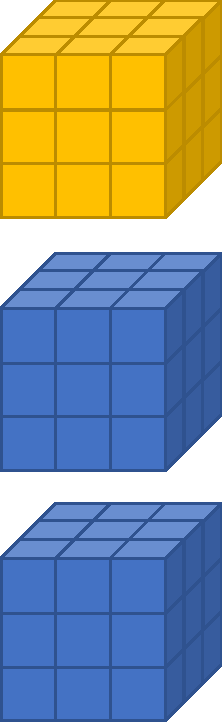
\includegraphics[width=0.33\linewidth]{filterwise.pdf}
    \caption{kernel-wise pruning}
    \label{fig:struct_pruning:fw}
    \end{subfigure}
    %
    \begin{subfigure}{.32\textwidth}
    \centering
    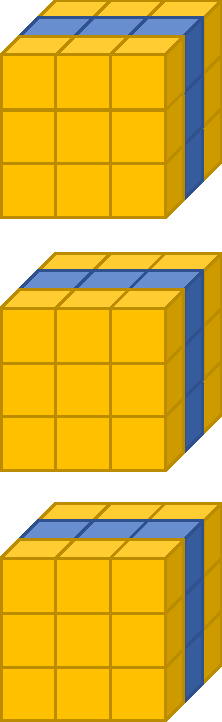
\includegraphics[width=0.33\linewidth]{channelwise.pdf}
    \caption{channel-wise pruning}
    \label{fig:struct_pruning:chw}
    \end{subfigure}
    %
    \begin{subfigure}{.32\textwidth}
    \centering
    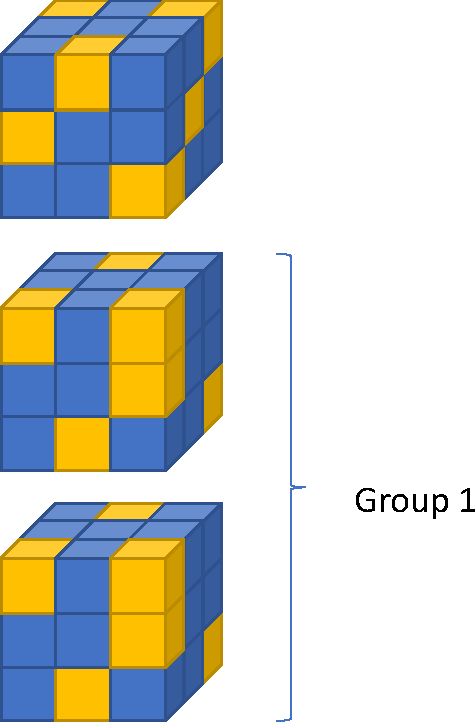
\includegraphics[width=0.70\linewidth]{shapewise.pdf}
    \caption{shape-wise pruning}
    \label{fig:struct_pruning:sw}
    \end{subfigure}
    %
    \caption{Structured pruning schemes, where the yellow weights are the pruned one}
    \label{fig:struct_pruning}
\end{figure}
%
Some works have focused on improving the speed of lightweight models with pruning. \textcite{zhang_channel_2019, tu_pruning_2019} have combined depthwise separable convolution and pruning. They both have chosen \textbf{Channel-wise} pruning because it does not create sparse connection and improves greatly the speed. It reduces also the computational complexity of the pointwise convolution (where the main arithmetic complexity is concentrated) and allows to avoid the depthwise convolution of the pruned channels too. Moreover, we can prune the pointwise kernel producting that channel in the previous block. We can see the process on figure \ref{toBeInserted}. 

In this work we focus on a structured pruning scheme for depthwise separable convolution. More precisely, we develop an architecture on \acrshort{fpga} than combine both advantages of pruning and depthwise separable convolution.0
%
%
\subsubsection{Quantization} \label{subs:quantization}
The approach of quantization is to compress (reducing the bit-width) of floating point parameters to fixed point low-precision parameters. The benefits of quantization, as enonced by \cite{joos_de_ter_beerst_accelerating_2019}, are a reduction of overfitting and an acceleration of computation because the weights have a smaller bit-size. For example, operations can be four 4 times faster when quantizing to 8 bits due to \acrshort{simd} optimisations.

There are two forms of quantization:
\begin{enumerate}
    \item \textbf{Fixed-point integers}: a number representation using bits is divided into two parts: the first part is dedicated to the integer part and the second one is dedicated to the fractional part of the number. It is easy to implement but it is important to consider the bit size of each part. It can be done by examination after the training. We can also, as for \cite{qiu_going_2016, yin_high_2018}, choose a different range for each layer (doing it for every weight is not memory-efficient).
    \item \textbf{Inteval quantification}: we redefine weights to be between $[-\alpha; \alpha]$. We have to retrain a network before using it but we can achieve good results with a small number of bits. If we fine-tune the network, we can even use 1 (Binary-wheight networks \cite{courbariaux_binarized_2016}) or 2 bits (Ternary-weight networks \cite{li_ternary_2016}).
\end{enumerate}
%
It was only recently that work are published on highly quantized \acrshort{nn} \cite{guo_survey_2018}, and using 16-bits or 8-bits quantization has shown only a small loss in accuracy without retraining \cite{abdelouahab_accelerating_2018}. The quantization of a \acrshort{nn} can be achieved through two different approaches:
\begin{enumerate}
    \item \textbf{Quantification of the weight parameters}: the most widely used. It can be done before or after training, but we have a better accuracy if we train during training.
    \item \textbf{Quantification through the activation layer}: we quantize the the output of the activation function;
\end{enumerate}
As pointed by \textcite{han_deep_2016}, quantization techniques and pruning are orthogonal and can be combined to compress further the network. Unfortunately, not all existing network are friendly for quantization, like MobileNetV1. There is a accuracy gap against float point models (70.50\% vs 1.80\% using a 8-bit pipeline). However, works of \textcite{sheng_quantization-friendly_2018} have shown that the source of accuracy drap was the design of the separable convolution core layer. They have therefore proposed a new quantization-friendly separable convolution core layer. Works on MobileNetV2 should then be done to verify the fixed-point inference accuracy. Still, MobileNet had a problem with 8-bit pipeline, increasing the bitwidth to 16-bit could boost accuracy \cite{cheng_recent_2018} and this bitwidth is widely used \cite{huimin_li_high_2016, bai_cnn_2018}. Therefore, 16-bit fixed point is adopted for input data, weight and intermediate data.
